\documentclass[12pt]{article}

\usepackage[utf8]{inputenc}
\usepackage[spanish]{babel}
\usepackage{amssymb, amsmath, geometry, graphicx}

\setlength{\parindent}{0cm}
\geometry{margin=2.54cm}
\decimalpoint
\pagestyle{plain}

\title{Ecuaciones paramétricas de algunas curvas y su representación gráfica}
\date{19 de junio de 2026}
\author{Rosendo Camal}

\begin{document}
\maketitle

% Actividad 1
\section*{Actividad 1}

\textbf{Instrucciones:} Construir la tabla de valores para $x = t$ y $y = t^2$ usando $t = -3, -2, -1, 0, 1, 2, 3$.
\newline

\textbf{Respuesta:}

\begin{center}
\begin{tabular}{| c | c | r |}
	\hline
	$t$ & $x$ & $y$ \\ \hline
	$-3$ & $-3$ & $(-3)^2 = 9$ \\
	$-2$ & $-2$ & $(-2)^2 = 4$ \\
	$-1$ & $-1$ & $(-1)^2 = 1$ \\
	$0$ & $0$ & $0^2 = 0$ \\
	$1$ & $1$ & $1^2 = 1$ \\
	$2$ & $2$ & $2^2 = 4$ \\
	$3$ & $3$ & $3^2 = 9$ \\ \hline
\end{tabular}
\end{center}

\begin{figure}[htb]
	\center
	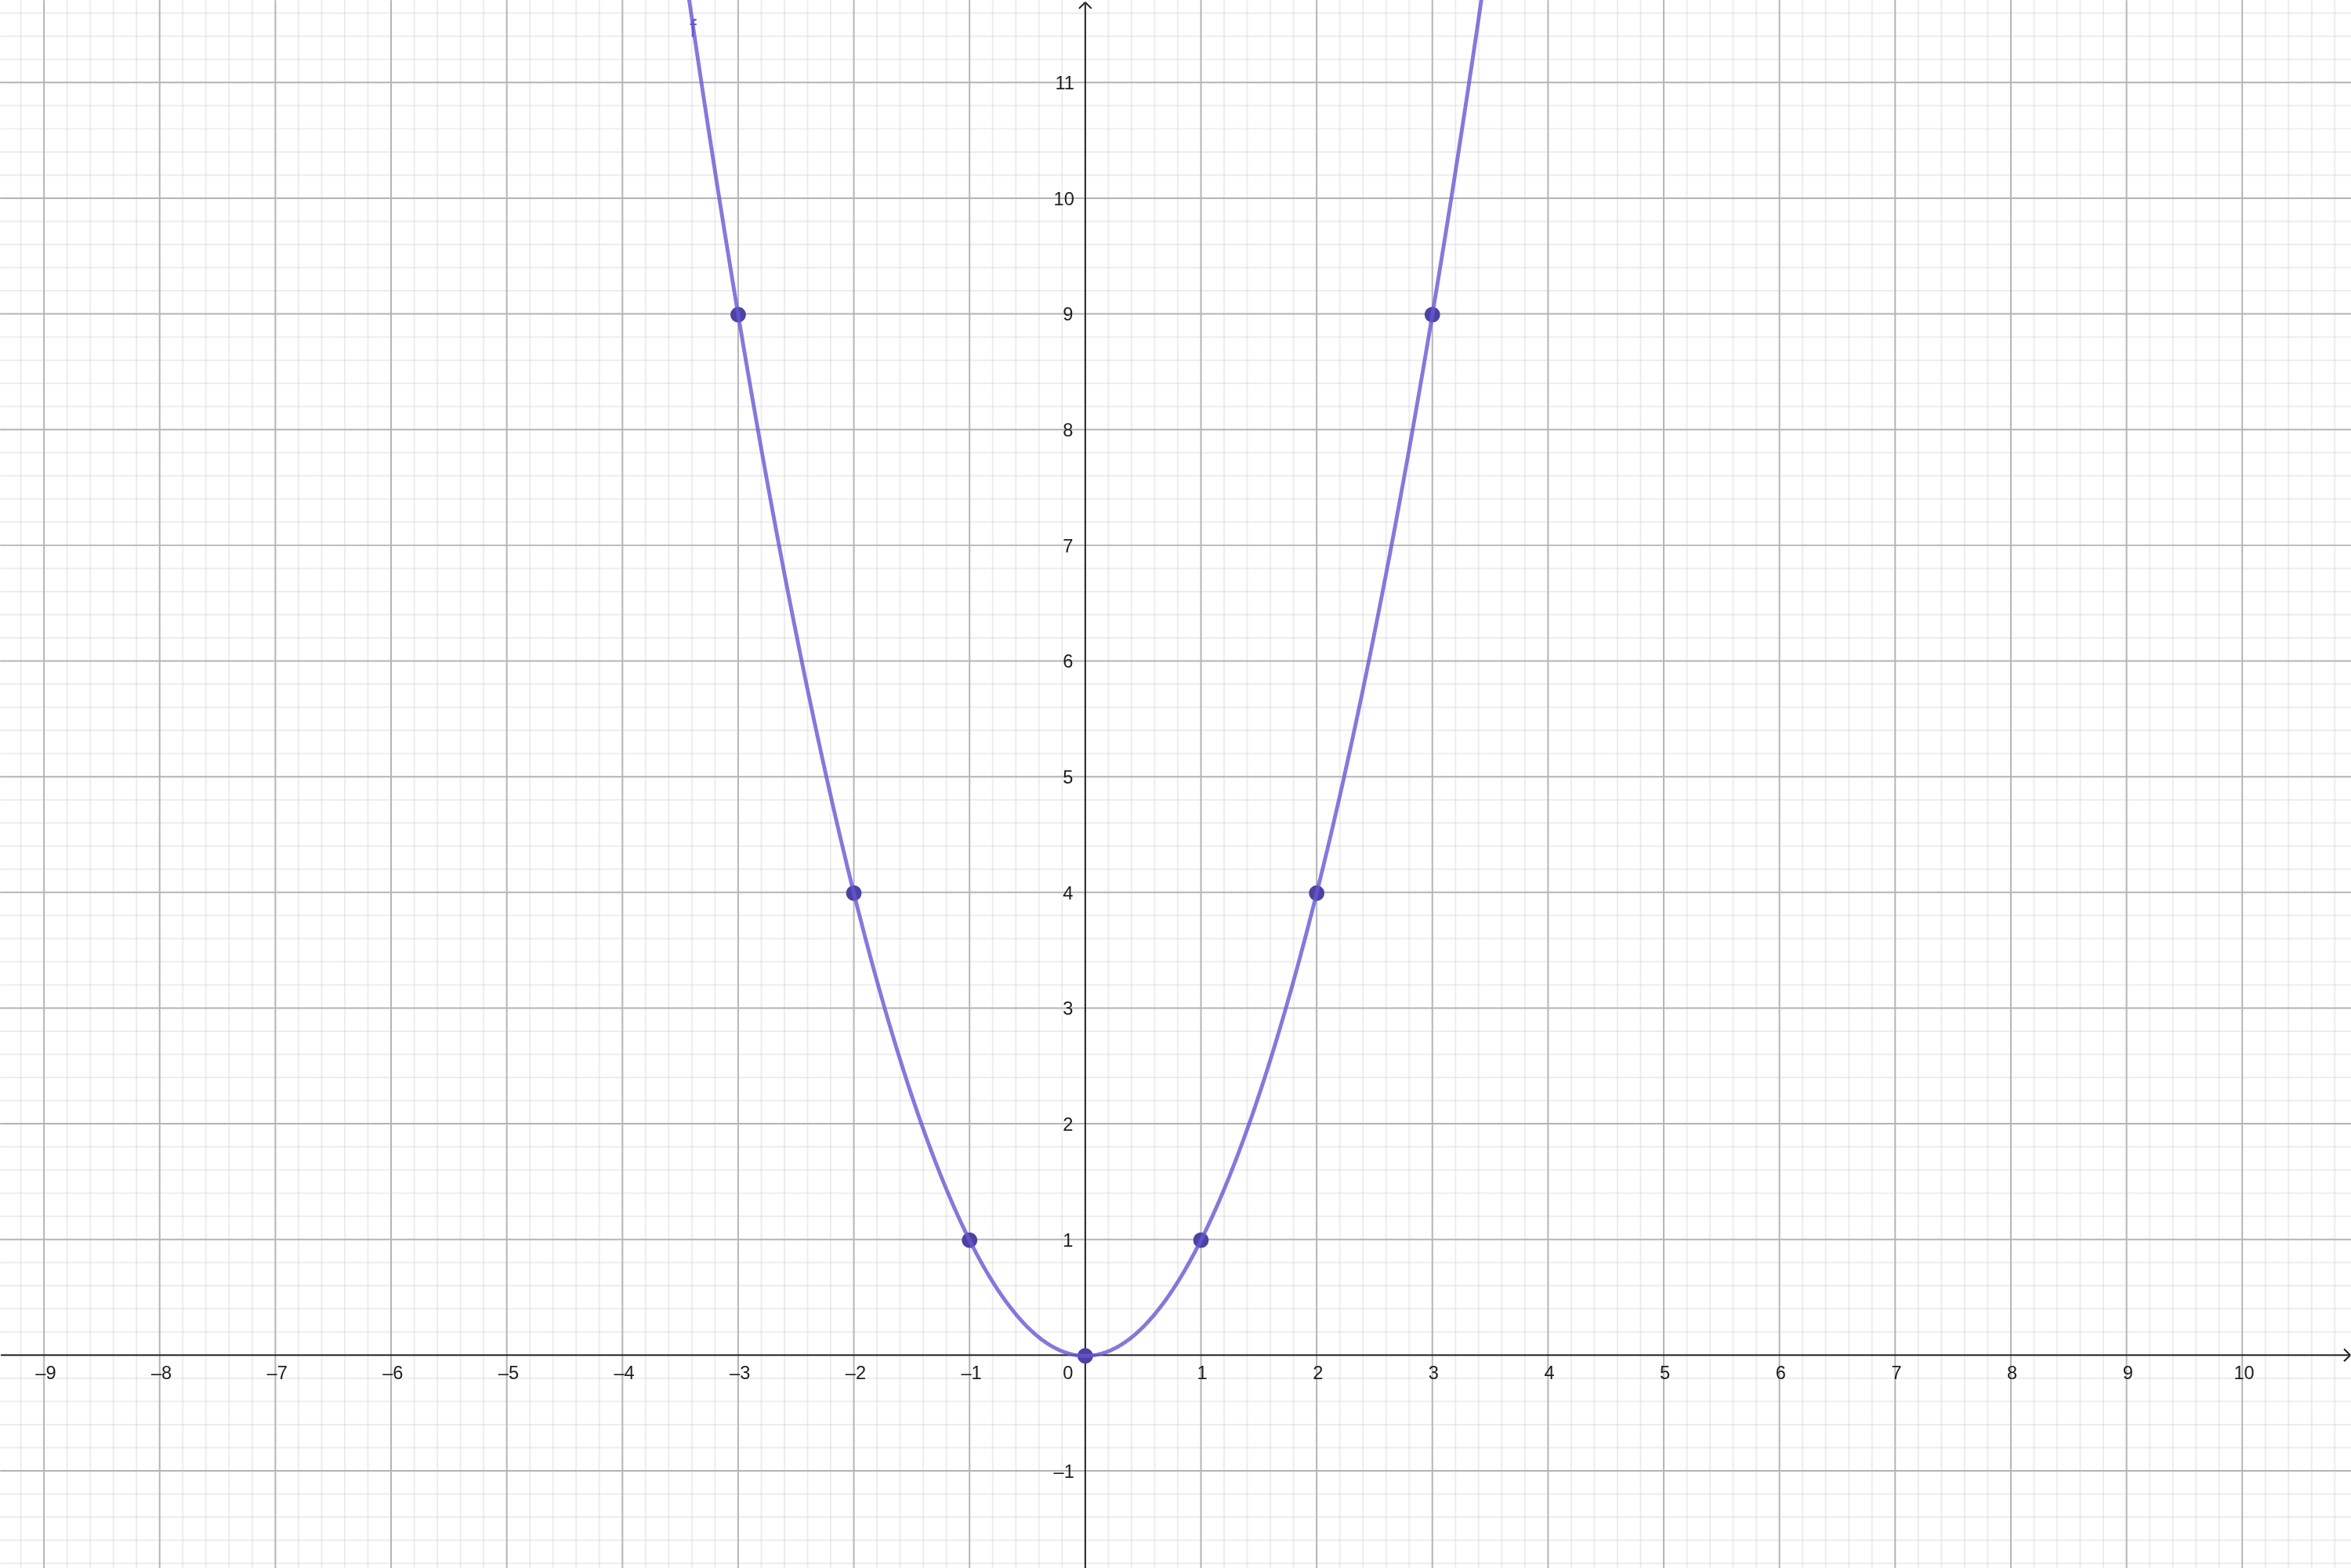
\includegraphics[width=0.7\linewidth]{./geogebra-export1.png}
\end{figure}
\newpage

% Actividad 2
\section*{Actividad 2}
\textbf{Instrucciones:} Determinar los puntos de la circuferencia $x = 4\cos(t)$ y $y = 4 \sin(t)$ para $t = 0^\circ, 90^\circ, 180^\circ, 270^\circ$.
\newline

\textbf{Respuesta:}

\begin{center}
\begin{tabular}{| c | c | c | c |}
	\hline
	$t$ & $x$ & $y$ & $(x, y)$ \\ \hline
	$0^\circ$ & $4\cos(0^\circ) = 4$ & $4\sin(0^\circ) = 0$ & $(4, 0)$ \\
	$90^\circ$ & $4\cos(90^\circ) = 0$ & $4\sin(90^\circ) = 4$ & $(0, 4)$ \\
	$180^\circ$ & $4\cos(180^\circ) = -4$ & $4\sin(180^\circ) = 0$ & $(-4, 0)$ \\
	$270^\circ$ & $4\cos(270^\circ) = 0$ & $4\sin(270^\circ) = -4$ & (0, -4) \\ \hline
\end{tabular}
\end{center}

\begin{figure}[htb]
	\center
	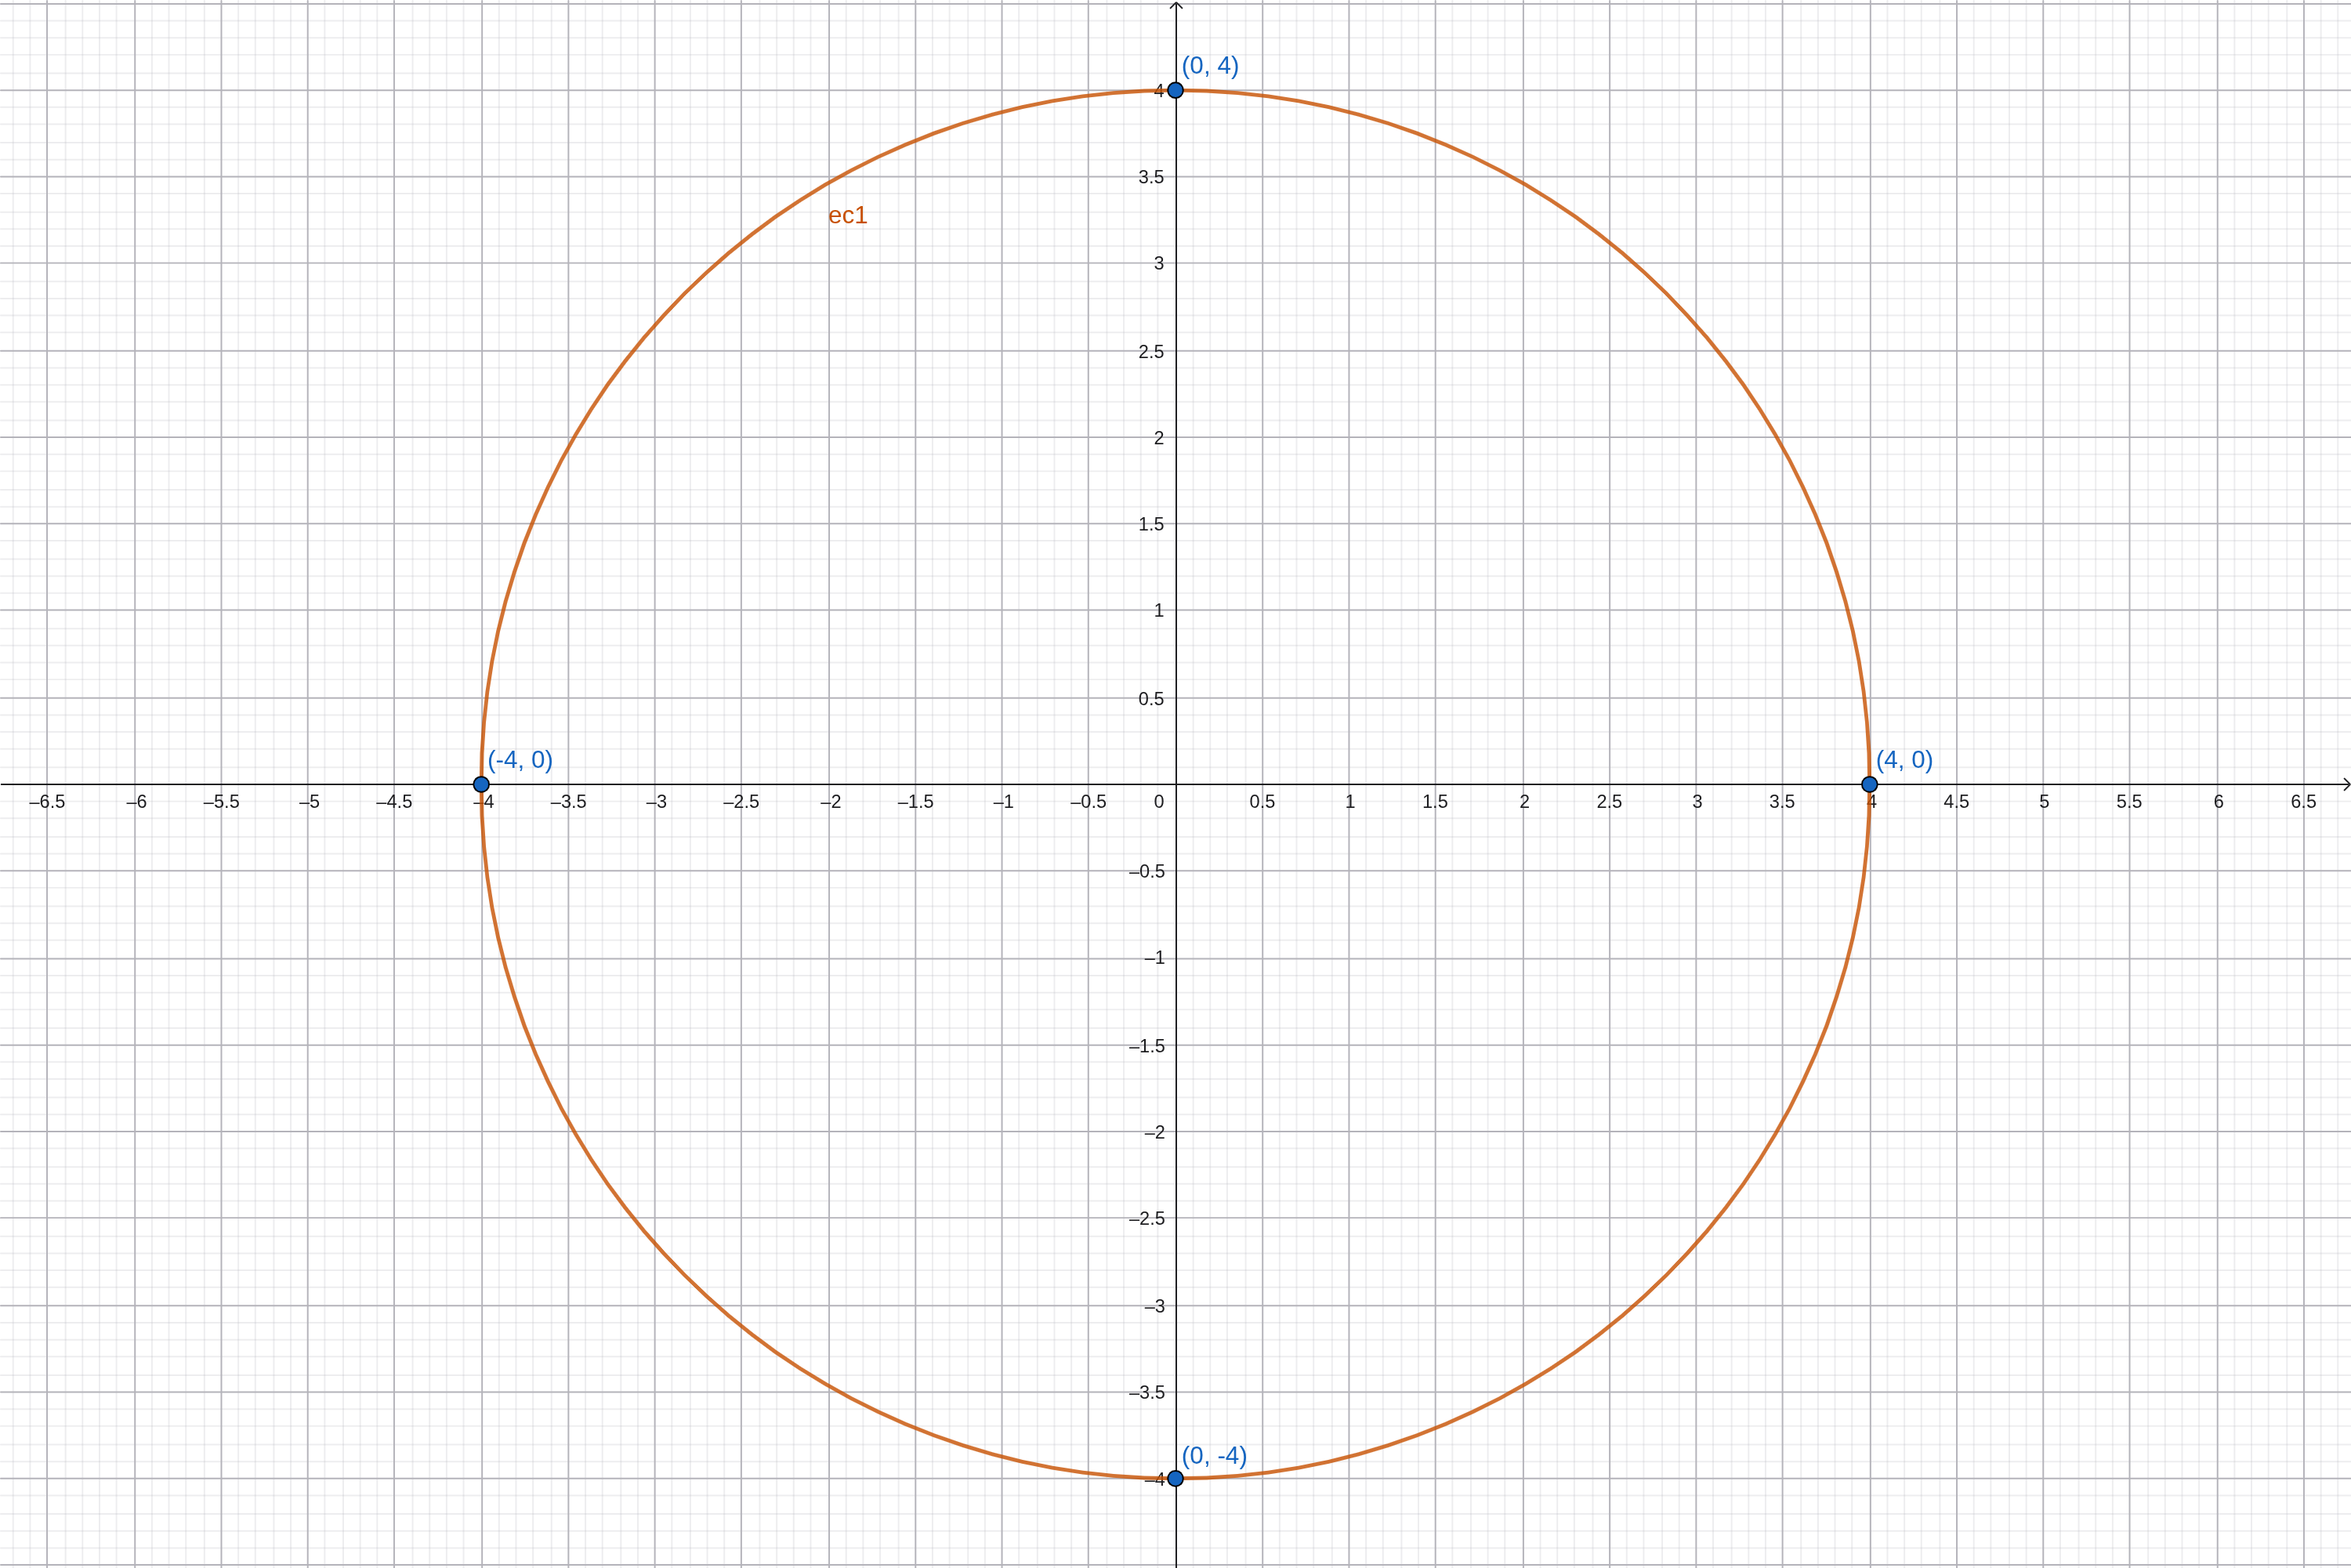
\includegraphics[width=0.7\linewidth]{./geogebra-export2.png}
\end{figure}
\newpage

% Actividad 3
\section*{Actividad 3}
\textbf{Instrucciones:} Graficar la elipse con $x = 6\cos(t)$ y $y = 2\sin(t)$ utilizando al menos ocho valores de $(t)$.
\newline

\textbf{Respuesta:}

\begin{center}
\begin{tabular}{| c | l | l | c |}
	\hline
	$t$ & $x$ & $y$ & $(x, y)$ \\ \hline
	$0$ & $6\cos(0) = 6$ & $2\sin(0) = 0$  & $(6, 0)$ \\
	$\pi\over4$ & $6\cos\left(\frac{\pi}{4}\right) \approx 4.24...$ & $2\sin\left(\frac{\pi}{4}\right) \approx 1.41...$ & $(4.24, 1.41)$ \\
	$\pi\over2$ & $6\cos\left(\frac{\pi}{2}\right) = 0$ & $2\sin\left(\frac{\pi}{2}\right) = 2$ & $(0, 2)$ \\
	$3\pi\over4$ & $6\cos\left(\frac{3\pi}{4}\right) \approx -4.24...$ & $2\sin\left(\frac{3\pi}{4}\right) \approx 1.41...$ & $(-4.24, 1.41)$ \\
	$\pi$ & $6\cos(\pi) = -6$ & $2\sin(\pi) = 0$ & $(-6, 0)$ \\
	$5\pi\over4$ & $6\cos\left(\frac{5\pi}{4}\right) \approx -4.24...$ & $2\sin\left(\frac{5\pi}{4}\right) \approx -1.41...$ & $(-4.24, -1.41)$ \\
	$3\pi\over2$ & $6\cos\left(\frac{3\pi}{2}\right) = 0$ & $2\sin\left(\frac{3\pi}{2}\right) = -2$ & $(0, -2)$ \\
	$7\pi\over4$ & $6\cos\left(\frac{7\pi}{4}\right) \approx 4.24...$ & $2\sin\left(\frac{7\pi}{4}\right) \approx -1.41...$ & $(4.24, -1.41)$ \\ \hline
\end{tabular}
\end{center}

\begin{figure}[htb]
	\center
	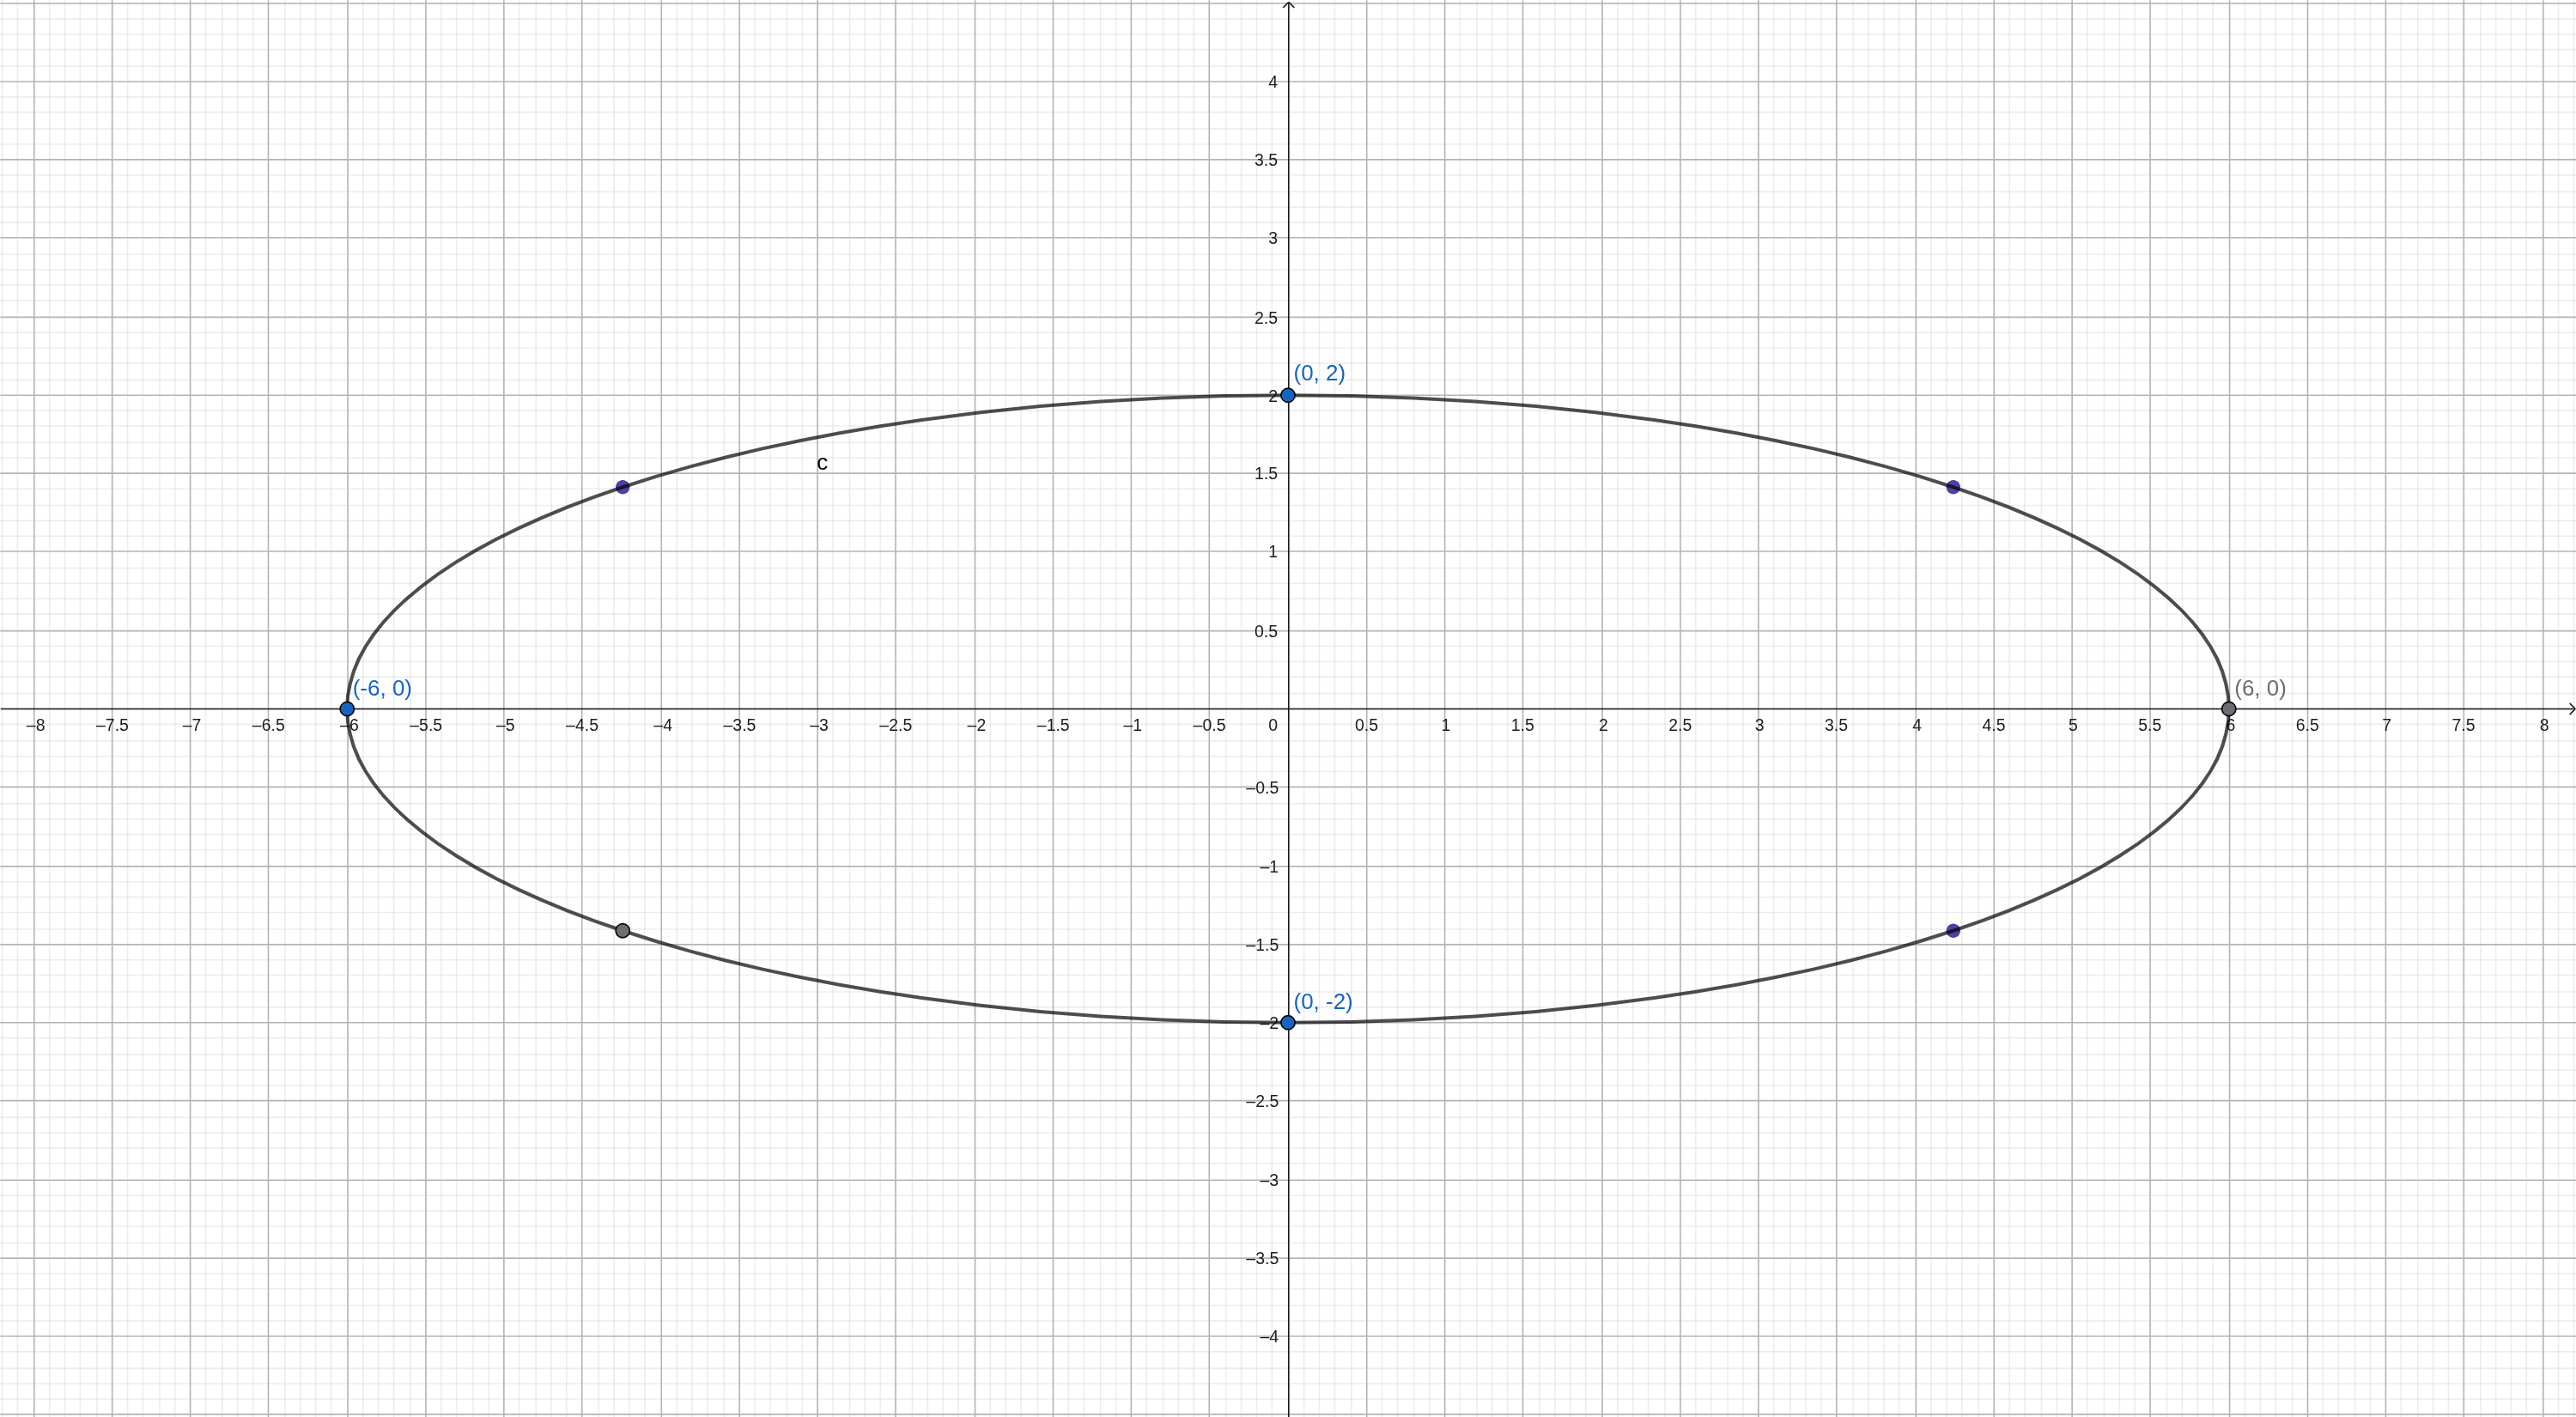
\includegraphics[width=0.7\linewidth]{./geogebra-export3.png}
\end{figure}

\end{document}
